\documentclass[a4paper, 11pt, titlepage]{article}
\usepackage{fancyhdr}
\usepackage{graphicx}
\usepackage{imakeidx}
\usepackage{makeidx}
\usepackage{mathtools}
\usepackage[spanish]{babel}
\usepackage{eurosym}
\usepackage{hyperref}
\usepackage{amssymb}
\usepackage{listings}
\usepackage{xcolor}
\usepackage{mathtools}
\usepackage{blkarray, bigstrut}

\title{Tecnología de computadores}
\author{Francisco Javier Balón Aguilar}

\begin{document}

\maketitle
\renewcommand{\contentsname}{Índice}
\tableofcontents
\newpage

\section{Álgebra de Boole y puertas lógicas}

    El matemático y filósofo George Boole enunció una teoría matemática que permitía, de forma 
    algebráica, representar y operar con lógica preposicional. Una de sus características más 
    importantes es que las variables sólo podían tener dos valores: verdadero y falso. A esta 
    teoría se le conoce como Álgebra de Boole.

    Posteriormente, Claude E. Shannon, ingeniero electrónico, llega a la conclusión de que 
    es posible aplicar el Álgebra de Boole para el diseño, estudio y simplificación de circuitos 
    digitales. Uno de los factores que lo permiten son la simplificación a dos los valores de 
    las variables.

    El Álgebra de Boole queda definida, pues, por las siguientes reglas:

    \begin{itemize}
        \item Las variables sólo tienen dos posibles valores: 0 ó 1, es decir, utilizamos el 
        sistema de numeración binario.
        \item Operación de complementación o función NOT.
        \item Operación de suma lógica o función OR.
        \item Operación de producto lógico o función AND.
        \item Por convenio, el producto lógico es precedente a la suma lógica.
    \end{itemize}

    Estas operaciones algebráicas se implementan en los circuitos digitales mediante \textbf{puertas 
    lógicas}. Cada operación tiene asignada una puerta lógica.

    % TODO: poner gráfica con la representación de las puertas lógicas.

    Para representar los posibles resultados de la función lógica en función de las entradas se 
    utilizan las \textbf{tablas de verdad}. Ésta consta de una serie de columnas que representan 
    las variables de entrada y de salida, representando todas las combinaciones posibles de entradas.

    \begin{figure}[htp]
      \centering
      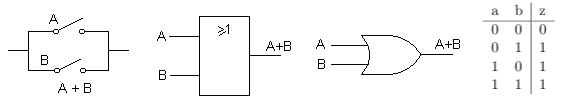
\includegraphics[width=1\textwidth]{resources/boole-or.png}
      \caption{Representación gráfica y tabla de verdad de la puerta lógica OR.}
      \label{boole-or}
    \end{figure}

    \begin{figure}[htp]
      \centering
      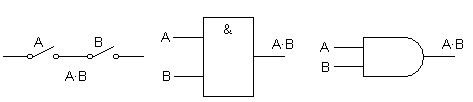
\includegraphics[width=1\textwidth]{resources/boole-and.png}
      \caption{Representación gráfica y tabla de verdad de la puerta lógica AND.}
      \label{boole-and}
    \end{figure}

    \begin{figure}[htp]
      \centering
      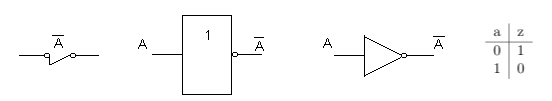
\includegraphics[width=1\textwidth]{resources/boole-not.png}
      \caption{Representación gráfica y tabla de verdad de la puerta lógica NOT.}
      \label{boole-not}
    \end{figure}

    \begin{figure}[htp]
      \centering
      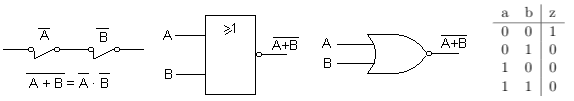
\includegraphics[width=1\textwidth]{resources/boole-nor.png}
      \caption{Representación gráfica y tabla de verdad de la puerta lógica NOR.}
      \label{boole-nor}
    \end{figure}

    \begin{figure}[htp]
      \centering
      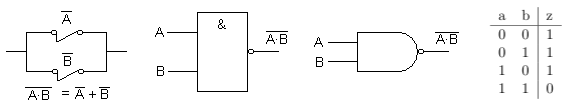
\includegraphics[width=1\textwidth]{resources/boole-nand.png}
      \caption{Representación gráfica y tabla de verdad de la puerta lógica NAND.}
      \label{boole-nand}
    \end{figure}

    \begin{figure}[htp]
      \centering
      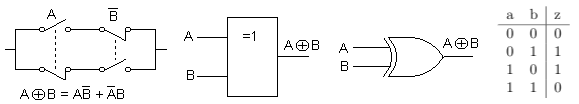
\includegraphics[width=1\textwidth]{resources/boole-xor.png}
      \caption{Representación gráfica y tabla de verdad de la puerta lógica XOR.}
      \label{boole-xor}
    \end{figure}


\end{document}